\PassOptionsToPackage{unicode=true}{hyperref} % options for packages loaded elsewhere
\PassOptionsToPackage{hyphens}{url}
\documentclass[11pt,dvipsnames,ignorenonframetext,aspectratio=169]{beamer}
\IfFileExists{pgfpages.sty}{\usepackage{pgfpages}}{}
\setbeamertemplate{caption}[numbered]
\setbeamertemplate{caption label separator}{: }
\setbeamercolor{caption name}{fg=normal text.fg}
\beamertemplatenavigationsymbolsempty
\usepackage{lmodern}
\usepackage{amssymb,amsmath}
\usepackage{ifxetex,ifluatex}
\usepackage{fixltx2e} % provides \textsubscript
\ifnum 0\ifxetex 1\fi\ifluatex 1\fi=0 % if pdftex
  \usepackage[T1]{fontenc}
  \usepackage[utf8]{inputenc}
\else % if luatex or xelatex
  \ifxetex
    \usepackage{mathspec}
  \else
    \usepackage{fontspec}
\fi
\defaultfontfeatures{Ligatures=TeX,Scale=MatchLowercase}







\fi

  \usetheme[]{monash}

  \usecolortheme{monashwhite}


% A default size of 24 is set in beamerthememonash.sty

% Title page
\setbeamertemplate{title page}
{\placefig{-0.01}{-0.01}{width=1.01\paperwidth,height=1.01\paperheight}{sissooleafwaterdrops.jpg}
% \begin{textblock}{7.5}(1,2.8)\usebeamerfont{title} % original
\begin{textblock}{15}(1,2.2)\usebeamerfont{title}
{\color{white}\raggedright\par\inserttitle}
\end{textblock}
\begin{textblock}{10}(1,6)
\small
{\color{white}\raggedright{\insertauthor}\mbox{}\\[0.1cm]
\insertdate}
\end{textblock}}


  \useinnertheme{rounded}

  \useoutertheme{smoothtree}

% use upquote if available, for straight quotes in verbatim environments
\IfFileExists{upquote.sty}{\usepackage{upquote}}{}
% use microtype if available
\IfFileExists{microtype.sty}{%
  \usepackage{microtype}
  \UseMicrotypeSet[protrusion]{basicmath} % disable protrusion for tt fonts
}{}


\newif\ifbibliography


\hypersetup{
      pdftitle={Geoinformatics: definition, concepts, tools and techniques and issues in Nepalease agriculture},
            colorlinks=true,
    linkcolor=red,
    citecolor=Blue,
    urlcolor=lightgrayd,
    breaklinks=true}
%\urlstyle{same}  % Use monospace font for urls







% Prevent slide breaks in the middle of a paragraph:
\widowpenalties 1 10000
\raggedbottom

  \AtBeginPart{
    \let\insertpartnumber\relax
    \let\partname\relax
    \frame{\partpage}
  }
  \AtBeginSection{
    \ifbibliography
    \else
      \let\insertsectionnumber\relax
      \let\sectionname\relax
      \frame{\sectionpage}
    \fi
  }
  \AtBeginSubsection{
    \let\insertsubsectionnumber\relax
    \let\subsectionname\relax
    \frame{\subsectionpage}
  }



\setlength{\parindent}{0pt}
\setlength{\parskip}{6pt plus 2pt minus 1pt}
\setlength{\emergencystretch}{3em}  % prevent overfull lines
\providecommand{\tightlist}{%
  \setlength{\itemsep}{0pt}\setlength{\parskip}{0pt}}

  \setcounter{secnumdepth}{0}


%% Monash overrides
\AtBeginSection[]{
   \frame<beamer>{
   \frametitle{Outline}\vspace*{0.2cm}
   
   \tableofcontents[currentsection,hideallsubsections]
  }}

% Redefine shaded environment if it exists (to ensure text is black)
\ifcsname Shaded\endcsname
  \definecolor{shadecolor}{RGB}{225,225,225}
  \renewenvironment{Shaded}{\color{black}\begin{snugshade}\color{black}}{\end{snugshade}}
\fi
%%

  \usepackage{setspace}
  \usepackage{wasysym}
  % \usepackage{footnote} % don't use this this breaks all
  \usepackage{fontenc}
  \usepackage{fontawesome}
  \usepackage{booktabs,siunitx}
  \usepackage{longtable}
  \usepackage{array}
  \usepackage{multirow}
  \usepackage{wrapfig}
  \usepackage{float}
  \usepackage{colortbl}
  \usepackage{pdflscape}
  \usepackage{tabu}
  \usepackage{threeparttable}
  \usepackage{threeparttablex}
  \usepackage[normalem]{ulem}
  \usepackage{makecell}
  \usepackage{xcolor}
  \usepackage{tikz} % required for image opacity change
  \usepackage[absolute,overlay]{textpos} % for text formatting
  \usepackage{chemfig}
  \usepackage[skip=0.333\baselineskip]{caption}
  % \newcommand*{\AlignChar}[1]{\makebox[1ex][c]{\ensuremath{\scriptstyle#1}}}%

  % this font option is amenable for beamer
  \setbeamerfont{caption}{size=\tiny}
  \singlespacing
  \definecolor{lightgrayd}{gray}{0.95}
  \definecolor{skyblued}{rgb}{0.65, 0.6, 0.94}
  \definecolor{oranged}{RGB}{245, 145, 200}

  \newlength{\cslhangindent}
  \setlength{\cslhangindent}{1.5em}
  \newenvironment{cslreferences}%
    {\setlength{\parindent}{0pt}%
    \everypar{\setlength{\hangindent}{\cslhangindent}}\ignorespaces}%
    {\par}

  \title[]{Geoinformatics: definition, concepts, tools and techniques
and issues in Nepalease agriculture}


  \author[
        Deependra Dhakal\\
Assistant Professor\\
\textit{ddhakal.rookie@gmail.com}\\
\url{https://rookie.rbind.io}
    ]{Deependra Dhakal\\
Assistant Professor\\
\textit{ddhakal.rookie@gmail.com}\\
\url{https://rookie.rbind.io}}


\date[
      
  ]{
    }

\begin{document}

% Hide progress bar and footline on titlepage
  \begin{frame}[plain]
  \titlepage
  \end{frame}


   \frame<beamer>{
   \frametitle{Outline}\vspace*{0.2cm}
   
   \tableofcontents[hideallsubsections]
  }

\hypertarget{geoinformatics}{%
\section{Geoinformatics}\label{geoinformatics}}

\begin{frame}{Meaning and definition}
\protect\hypertarget{meaning-and-definition}{}
\begin{itemize}
\tightlist
\item
  Science and technology dealing with the structure and character of
  spatial information, its capture, its classification and
  quantification, its storage, processing, portrayal and dissemination,
  including the infrastructure necessary to secure optimal use of this
  information.
\item
  Categorized under technical geography
\item
  Relies upon the theory and practical implications of geodesy.
\item
  Geography and earth science increasingly rely on digital spatial data
  acquired from remotely sensed images analyzed by geographical
  information systems (GIS), photo interpretation of aerial photographs
\end{itemize}
\end{frame}

\begin{frame}{}
\protect\hypertarget{section}{}
\begin{itemize}
\tightlist
\item
  For analysis of geographic information:

  \begin{itemize}
  \tightlist
  \item
    geospatial analysis and modeling (geocomputation),
  \item
    geovisualization
  \end{itemize}
\item
  Also deals with:

  \begin{itemize}
  \tightlist
  \item
    development of geospatial databases,
  \item
    information systems design,
  \item
    human-computer interaction and
  \item
    wired and wireless networking technologies
  \end{itemize}
\end{itemize}
\end{frame}

\begin{frame}{Areas of geoinformatics}
\protect\hypertarget{areas-of-geoinformatics}{}
\begin{itemize}
\tightlist
\item
  Cartography
\item
  Geodesy
\item
  Satellite navigation
\item
  Photogrammetry
\item
  Remote sensing
\item
  Spatial analysis
\item
  Web mapping
\item
  Navigation
\end{itemize}
\end{frame}

\begin{frame}{Digital earth}
\protect\hypertarget{digital-earth}{}
\footnotesize

\begin{itemize}
\tightlist
\item
  Digital Earth is the name given to a concept coined by former US vice
  president Al Gore in 1998, that describes a virtual representation of
  the Earth that is spatially referenced and interconnected with the
  world's digital knowledge archives. Furthermore, the greater part of
  this knowledge store would be free to all via internet.
\item
  The global dimension of the digital earth concept is perhaps best
  captured by two excerpts from Beijing declaration on digital Earth:

  \begin{itemize}
  \scriptsize
  \item Digital earth is an integral part of other advanced technologies including: Earth observation, geo-information system, global positioning systems, communication networks, sensor webs, electromagnetic identifiers, virtual reality, grid computation, etc. It is seen as a global strategic contributer to scientific and technological developments, and will be a catalyst in finding solutions to international scientific and societal issues;
  \item Digital earth should play a strategic and sustainable role in addressing such challenges to human society as natural resource depletion, food and water insecurity, energy shortages, environmental degradation, natural disaster response, population explosion, and, in particular, global climate change.
  \end{itemize}
\end{itemize}
\end{frame}

\begin{frame}{}
\protect\hypertarget{section-1}{}
\begin{figure}

{\centering 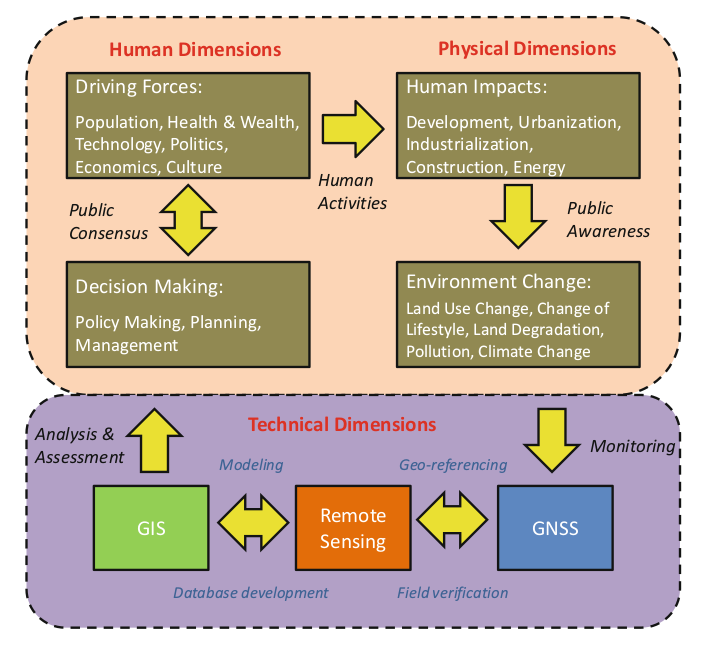
\includegraphics[width=0.65\linewidth]{../images/framework_geoinformatics} 

}

\caption{Conceptual framework for wide applications of geo-informatics}\label{fig:conceptual-framework-geoinformatics}
\end{figure}
\end{frame}

\begin{frame}{Applications}
\protect\hypertarget{applications}{}
\begin{columns}[T, onlytextwidth]
\column{0.5\textwidth}
\begin{itemize}
\item Urban planning and land use management,
\item in-car navigation systems,
\item virtual globes,
\item public health,
\item local and national territory management,
\item environmental modeling and analysis,
\item military,
\item transport network planning and management,
\item agriculture,
\end{itemize}
\column{0.5\textwidth}
\begin{itemize}
\item meteorology and climate change,
\item oceanography and atmosphere modeling,
\item business location planning,
\item architecture and archaeological reconstruction,
\item telecommunications,
\item criminology and crime simulation,
\item aviation and maritime transport
\item biodiversity conservation
\end{itemize}
\end{columns}
\end{frame}

\hypertarget{tools-and-techniques}{%
\section{Tools and techniques}\label{tools-and-techniques}}

\begin{frame}{Cartography}
\protect\hypertarget{cartography}{}
\begin{itemize}
\tightlist
\item
  Study and practice of making and using maps. Combining science and
  aesthetics and technique, cartography builds on the premise that
  reality can be modeled in ways that communicate spatial information
  effectively.
\item
  Coordinate reference system defines how the visual mapping of spatial
  data should be done

  \begin{itemize}
  \tightlist
  \item
    CRS has projection parameters, which is configurable giving a
    variation in mapping
    \footnote[frame]{\url{https://proj.org/usage/projections.html}}.
  \end{itemize}
\item
  Objectives of traditional cartography:

  \begin{itemize}
  \tightlist
  \item
    Set the map agenda and select traits (roads, land masses, political
    boundaries) of the object to be mapped.
  \item
    Represent the terrain of the mapped object on flat media
    (projection)
  \item
    Reduce the complexity (generalization).
  \item
    Organize the elements of the map to best convey its message (map
    design)
  \end{itemize}
\item
  Modern cartography constitutes theoretical and practical foundations
  of GIS and Geographic information
  science\footnote[frame]{Overview of CRS (in R) is available at: \url{https://www.nceas.ucsb.edu/sites/default/files/2020-04/OverviewCoordinateReferenceSystems.pdf}}.
\end{itemize}
\end{frame}

\begin{frame}{Map types}
\protect\hypertarget{map-types}{}
\begin{itemize}
\tightlist
\item
  General vs.~thematic cartography

  \begin{itemize}
  \tightlist
  \item
    General:

    \begin{itemize}
    \tightlist
    \item
      Intended for general audience and containing a variety of
      features. Bear many reference and location systems.
    \end{itemize}
  \item
    Thematic:

    \begin{itemize}
    \tightlist
    \item
      Specific geographic themes
    \item
      Oriented toward specific audiences
    \item
      Dot map showing corn production in different districts of Nepal
      divided into numerical choropleth classes.
    \item
      With the increasing volume of geographic data, thematic
      cartography has become increasingly useful and necessary to
      interpret spatial, cultural and social data
    \end{itemize}
  \end{itemize}
\end{itemize}
\end{frame}

\begin{frame}{General cartography}
\protect\hypertarget{general-cartography}{}
\begin{columns}[T, onlytextwidth]
\column{0.6\textwidth}


\includegraphics[width=0.95\linewidth]{03.4-geoinformatics_common_issues_files/figure-beamer/world-map-showing-nepal-1} 

\column{0.4\textwidth}


\includegraphics[width=0.98\linewidth]{03.4-geoinformatics_common_issues_files/figure-beamer/nepal-sf-dataframe-1} 

\end{columns}
\end{frame}

\begin{frame}{Thematic cartography}
\protect\hypertarget{thematic-cartography}{}
\begin{center}\includegraphics[width=0.66\linewidth]{03.4-geoinformatics_common_issues_files/figure-beamer/nepal-sf-dataframe-thematic-1} \end{center}
\end{frame}

\begin{frame}{Projections}
\protect\hypertarget{projections}{}
\begin{itemize}
\tightlist
\item
  Projections map the spherical 3D space to a flat 2D space
  \footnote[frame]{https://proj.org/usage/projections.html}.
\item
  Projections are coordinate operations that are technically conversions
  but since projections are so fundamental to PROJ we differentiate them
  from conversions.
\end{itemize}

\setlength{\tabcolsep}{2pt}

\begin{table}
\centering\begingroup\fontsize{4}{6}\selectfont

\begin{tabular}{>{\raggedright\arraybackslash}p{8em}>{\raggedright\arraybackslash}p{8em}>{\raggedright\arraybackslash}p{8em}>{\raggedright\arraybackslash}p{8em}>{\raggedright\arraybackslash}p{8em}>{\raggedright\arraybackslash}p{8em}>{\raggedright\arraybackslash}p{8em}>{\raggedright\arraybackslash}p{8em}>{\raggedright\arraybackslash}p{8em}>{\raggedright\arraybackslash}p{8em}}
\toprule
Projection & Projection & Projection & Projection & Projection & Projection & Projection & Projection & Projection & Projection\\
\midrule
Adams Hemisphere in a Square & Cassini (Cassini-Soldner) & Eckert VI & Modified Stereographic of 50 U & Laborde & McBryde-Thomas Flat-Polar Sinusoidal & New Zealand Map Grid & Putnins P4’ & Oblique Stereographic Alternative & van der Grinten II\\
Adams World in a Square I & Central Cylindrical & Equidistant Cylindrical (Plate Carrée) & Guyou & Lambert Azimuthal Equal Area & Mercator & General Oblique Transformation & Putnins P5 & Gauss-Schreiber Transverse Mercator (aka Gauss-Laborde Reunion) & van der Grinten III\\
Adams World in a Square II & Central Conic & Equidistant Conic & Hammer \& Eckert-Greifendorff & Lagrange & Miller Oblated Stereographic & Oblique Cylindrical Equal Area & Putnins P5’ & Transverse Central Cylindrical & van der Grinten IV\\
Albers Equal Area & Equal Area Cylindrical & Equal Earth & Hatano Asymmetrical Equal Area & Larrivee & Miller Cylindrical & Oblated Equal Area & Putnins P6 & Transverse Cylindrical Equal Area & Vitkovsky I\\
Azimuthal Equidistant & Chamberlin Trimetric & Euler & HEALPix & Laskowski & Space oblique for MISR & Oblique Mercator & Putnins P6’ & Times & Wagner I (Kavrayskiy VI)\\
\addlinespace
Airy & Collignon & Fahey & rHEALPix & Lambert Conformal Conic & Mollweide & Ortelius Oval & Quartic Authalic & Tissot & Wagner II\\
\bottomrule
\end{tabular}
\endgroup{}
\end{table}
\end{frame}

\begin{frame}{}
\protect\hypertarget{section-2}{}
\setlength{\tabcolsep}{2pt}

\begin{table}
\centering\begingroup\fontsize{4}{6}\selectfont

\begin{tabular}{>{\raggedright\arraybackslash}p{8em}>{\raggedright\arraybackslash}p{8em}>{\raggedright\arraybackslash}p{8em}>{\raggedright\arraybackslash}p{8em}>{\raggedright\arraybackslash}p{8em}>{\raggedright\arraybackslash}p{8em}>{\raggedright\arraybackslash}p{8em}>{\raggedright\arraybackslash}p{8em}>{\raggedright\arraybackslash}p{8em}>{\raggedright\arraybackslash}p{8em}}
\toprule
Projection & Projection & Projection & Projection & Projection & Projection & Projection & Projection & Projection & Projection\\
\midrule
Aitoff & Colombia Urban & Foucaut & Interrupted Goode Homolosine & Lambert Conformal Conic Alternative & Murdoch I & Orthographic & Quadrilateralized Spherical Cube & Transverse Mercator & Wagner III\\
Modified Stereographic of Alaska & Compact Miller & Foucaut Sinusoidal & Interrupted Goode Homolosine (Oceanic View) & Lambert Equal Area Conic & Murdoch II & Patterson & Robinson & Tobler-Mercator & Wagner IV\\
Apian Globular I & Craster Parabolic (Putnins P4) & Gall (Gall Stereographic) & Interrupted Mollweide & Lee Oblated Stereographic & Murdoch III & Perspective Conic & Roussilhe Stereographic & Two Point Equidistant & Wagner V\\
August Epicycloidal & Denoyer Semi-Elliptical & Geostationary Satellite View & Interrupted Mollweide (Oceanic View) & Loximuthal & Natural Earth & Peirce Quincuncial & Rectangular Polyconic & Tilted perspective & Wagner VI\\
Bacon Globular & Eckert I & Ginsburg VIII (TsNIIGAiK) & International Map of the World Polyconic & Space oblique for LANDSAT & Natural Earth II & Polyconic (American) & S2 & Universal Polar Stereographic & Wagner VII\\
\addlinespace
Bertin 1953 & Eckert II & General Sinusoidal Series & Icosahedral Snyder Equal Area & McBryde-Thomas Flat-Polar Sine (No & Nell & Putnins P1 & Spherical Cross-track Height & Urmaev V & Web Mercator / Pseudo Mercator\\
Bipolar conic of western hemisphere & Eckert III & Gnomonic & Kavrayskiy V & McBryde-Thomas Flat-Pole Sine (No & Nell-Hammer & Putnins P2 & Sinusoidal (Sanson-Flamsteed) & Urmaev Flat-Polar Sinusoidal & Werenskiold I\\
Boggs Eumorphic & Eckert IV & Goode Homolosine & Kavrayskiy VII & McBride-Thomas Flat-Polar Parabolic & Nicolosi Globular & Putnins P3 & Swiss Oblique Mercator & Universal Transverse Mercator (UTM) & Winkel I\\
Bonne (Werner lat\_1=90) & Eckert V & Modified Stereographic of 48 U & Krovak & McBryde-Thomas Flat-Polar Quartic & Near-sided perspective & Putnins P3’ & Stereographic & van der Grinten (I) & Winkel II\\
Cal Coop Ocean Fish Invest Lines/Stations &  &  &  &  &  &  &  &  & Winkel Tripel\\
\bottomrule
\end{tabular}
\endgroup{}
\end{table}
\end{frame}

\begin{frame}{}
\protect\hypertarget{section-3}{}
\footnotesize

EPSG codes for commonly used CRS (in the U.S.)

\begin{enumerate}
\tightlist
\item
  Latitude/Longitude

  \begin{itemize}
    \scriptsize
    \item WGS84 (EPSG: 4326)
    \item Commonly used by organizations that provide GIS data for the entire globe or many countries. CRS used by Google Earth
    \end{itemize}
\item
  NAD83 (EPSG:4269)

  \begin{itemize}
    \scriptsize
    \item Most commonly used by U.S. federal agencies.
    \end{itemize}
\item
  NAD27 (EPSG: 4267)

  \begin{itemize}
    \scriptsize
    \item Old version of NAD83
    \end{itemize}
\item
  Projected (Easting/Northing)

  \begin{itemize}
    \scriptsize
    \item UTM, Zone 10 (EPSG: 32610)
    \item Zone 10 is used in the Pacific Northwest
    \end{itemize}
\item
  Mercator (EPSG: 3857); Tiles from Google Maps, Open Street Maps,
  Stamen map
\end{enumerate}
\end{frame}

\begin{frame}{Universal Transverse Mercator}
\protect\hypertarget{universal-transverse-mercator}{}
\footnotesize

UTM coordinate comprises a zone number, a hemisphere (N/S), an easting
and a northing. Eastings are referenced from the central meridian of
each zone, \& northings from the equator, both in metres. To avoid
negative numbers, `false eastings' and `false northings' are used:

Eastings are measured from 500,000 metres west of the central meridian.
Eastings (at the equator) range from 166,021m to 833,978m (the range
decreases moving away from the equator); a point on the the central
meridian has the value 500,000m.

In the northern hemisphere, northings are measured from the equator -
ranging from 0 at the equator to 9,329,005m at 84 degree N). In the
southern hemisphere they are measured from 10,000,000 metres south of
the equator (close to the pole) - ranging from 1,116,915m at 80 degree S
to 10,000,000m at the equator.

Nepal lies in the UTM zone of 440N and 450N. The scale factor is 0.9996
for the central meridian. 10 49' east or west of central meridian has
the scale factor of 1.

\scriptsize

Norway/Svalbard: the designers of UTM made two exceptions to the rule.
The part of zone 31 covering western Norway is transferred to zone 32,
and the zones covering Svalbard are tweaked to keep Svalbard in two
zones (it's easier to understand looking at a map). These widened zones
are viable partly because zones are much narrower so far north, so
little precision is lost in merging them.
\end{frame}

\begin{frame}{}
\protect\hypertarget{section-4}{}
\begin{columns}[T, onlytextwidth]
\column{0.3\textwidth}


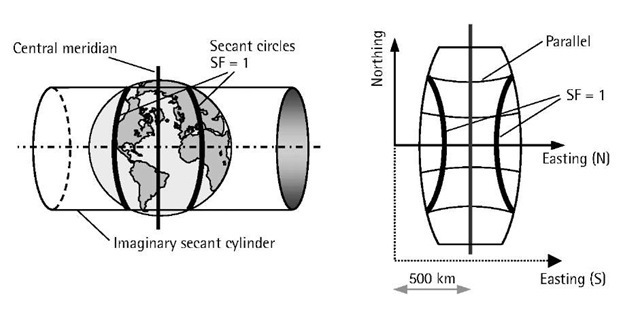
\includegraphics[width=0.99\linewidth]{../images/UTM_projection} 

\column{0.7\textwidth}

\begin{itemize}
\scriptsize
\item Traditionally Universal Transverse Mercator (UTM) Projection system has been in use in Nepal; Mercator projection is Conformal Cylindrical Projection.
\item In Transverse projection, Earth is wrapped around a cylinder in such a manner that point of tangency between Globe and Cylinder is a meridian, or line of longitude, called Central Meridian. In Conformal or Orthomorphic Projection, the shape/angle is preserved even though the length and breadth may distort.
\item UTM consists total of 60 zones of longitude each of 60 extending from 180 W to 180 E. 180 W to 174 W is designated as zone 1 with the central meridian of 177 W and other zone goes as so on and so further manner. Further zone are divided in rows with a difference of 8. These zone extend from 80 S Latitude to 84 N latitude. The first Latitude zone is designated with letter C for 80 S to 72 S latitude.
\item In recent years with cadastral survey and various accuracy techniques, Nepal has default projection set to MUTM (Modified UTM) -- a Gauss-Krueger projection-based coordinate system. In this system, earth is divided in 120 zones each of 3 degree.
\item Nepal has central meridian of 81 degree, 84 degree and 87 degree.
\item Scale factor of 0.9999 is used for central meridian normally for 84 degree and 0 degree 55 minutes east or west of central meridian has the scale factor of 1 (meaning no distortion).
\item False Easting at central meridian is 500,000 m in order to keep all the coordinates within the country positive, and False Northing at the Equator is 0 m.
\end{itemize}
\end{columns}
\end{frame}

\begin{frame}[fragile]{}
\protect\hypertarget{section-5}{}
\tiny

\begin{verbatim}
## Coordinate Reference System:
##   User input: EPSG:26919 
##   wkt:
## PROJCRS["NAD83 / UTM zone 19N",
##     BASEGEOGCRS["NAD83",
##         DATUM["North American Datum 1983",
##             ELLIPSOID["GRS 1980",6378137,298.257222101,
##                 LENGTHUNIT["metre",1]]],
##         PRIMEM["Greenwich",0,
##             ANGLEUNIT["degree",0.0174532925199433]],
##         ID["EPSG",4269]],
##     CONVERSION["UTM zone 19N",
##         METHOD["Transverse Mercator",
##             ID["EPSG",9807]],
##         PARAMETER["Latitude of natural origin",0,
##             ANGLEUNIT["degree",0.0174532925199433],
##             ID["EPSG",8801]],
##         PARAMETER["Longitude of natural origin",-69,
##             ANGLEUNIT["degree",0.0174532925199433],
##             ID["EPSG",8802]],
##         PARAMETER["Scale factor at natural origin",0.9996,
##             SCALEUNIT["unity",1],
##             ID["EPSG",8805]],
##         PARAMETER["False easting",500000,
##             LENGTHUNIT["metre",1],
##             ID["EPSG",8806]],
##         PARAMETER["False northing",0,
##             LENGTHUNIT["metre",1],
##             ID["EPSG",8807]]],
##     CS[Cartesian,2],
##         AXIS["(E)",east,
##             ORDER[1],
##             LENGTHUNIT["metre",1]],
##         AXIS["(N)",north,
##             ORDER[2],
##             LENGTHUNIT["metre",1]],
##     USAGE[
##         SCOPE["Engineering survey, topographic mapping."],
##         AREA["North America - between 72°W and 66°W - onshore and offshore. Canada - Labrador; New Brunswick; Nova Scotia; Nunavut; Quebec. Puerto Rico. United States (USA) - Connecticut; Maine; Massachusetts; New Hampshire; New York (Long Island); Rhode Island; Vermont."],
##         BBOX[14.92,-72,84,-66]],
##     ID["EPSG",26919]]
\end{verbatim}

\begin{verbatim}
## CRS arguments:
##  +proj=utm +zone=19 +datum=NAD83 +units=m +no_defs +ellps=GRS80
## +towgs84=0,0,0
\end{verbatim}

\normalsize
\end{frame}

\begin{frame}{}
\protect\hypertarget{section-6}{}
\begin{columns}
\column{0.5\textwidth}


\includegraphics[width=0.95\linewidth]{03.4-geoinformatics_common_issues_files/figure-beamer/map-projection-mercator-1} 

\column{0.5\textwidth}


\includegraphics[width=0.95\linewidth]{03.4-geoinformatics_common_issues_files/figure-beamer/map-projection-utm-1} 

\end{columns}
\end{frame}

\begin{frame}{}
\protect\hypertarget{section-7}{}
\begin{columns}
\column{0.5\textwidth}


\includegraphics[width=0.95\linewidth]{03.4-geoinformatics_common_issues_files/figure-beamer/map-projection-azimuthal-1} 

\column{0.5\textwidth}


\includegraphics[width=0.95\linewidth]{03.4-geoinformatics_common_issues_files/figure-beamer/map-projection-robinson-1} 

\end{columns}
\end{frame}

\begin{frame}{Use in precision agriculture}
\protect\hypertarget{use-in-precision-agriculture}{}
\begin{enumerate}
\tightlist
\item
  Agricultural mapping
\end{enumerate}

\begin{itemize}
\tightlist
\item
  Current and future variations in the rainfall
\item
  Crop output and temperature of the soil
\item
  Farm resource and structure mapping
\end{itemize}

\begin{enumerate}
\setcounter{enumi}{1}
\tightlist
\item
  Soil analysis
\end{enumerate}

\begin{itemize}
\tightlist
\item
  Mapping of soil type and crop suitability
\item
  Nutrient and fertilizer status mapping
\end{itemize}

\begin{enumerate}
\setcounter{enumi}{2}
\tightlist
\item
  Data combination
\end{enumerate}

\begin{itemize}
\tightlist
\item
  Realistic appraisal of farm production to assist insurance
\item
  Farmers could access data of their crops across the seasons to compare
  and contrast
\end{itemize}
\end{frame}

\begin{frame}{}
\protect\hypertarget{section-8}{}
\begin{enumerate}
\setcounter{enumi}{3}
\tightlist
\item
  Increased interaction
\end{enumerate}

\begin{itemize}
\tightlist
\item
  Humans have better sense of space and time than any other variables
\item
  Using machinery and GIS (including on-ground data), interventions
  could be more efficiently and effectively applied.
\end{itemize}

\begin{enumerate}
\setcounter{enumi}{4}
\tightlist
\item
  Assembly of information to develop systems based models
\end{enumerate}

\begin{itemize}
\tightlist
\item
  Various layers of information such as soil moisture, nutrients,
  elevation, topography, irradiance, cloud cover, etc. could aid in
  feeding into growth models
\item
  These could be translated into recommendation systems for precise
  implementation.
\end{itemize}
\end{frame}

\begin{frame}{}
\protect\hypertarget{section-9}{}
\begin{enumerate}
\setcounter{enumi}{5}
\tightlist
\item
  Real-time mapping
\item
  Raising alert and disaster mapping
\item
  Historical data comparison
\item
  Boosting production
\end{enumerate}
\end{frame}

\hypertarget{common-issues-and-concerns-of-geoinformatics-in-nepalese-agriculture}{%
\section{Common issues and concerns of geoinformatics in Nepalese
agriculture}\label{common-issues-and-concerns-of-geoinformatics-in-nepalese-agriculture}}

\begin{frame}{Current state}
\protect\hypertarget{current-state}{}
\begin{itemize}
\tightlist
\item
  GIS based technology has already permeated through engineering
  discipline and seen its applications.
\item
  Recently, natural resource management (forest, watershed) operations
  also have begun making use of geo-spatial data.

  \begin{itemize}
  \tightlist
  \item
    tracking of forest and shrubland coverage using geo-spatial data
  \item
    monitoring of wildlife species using GPS tracker
  \end{itemize}
\item
  Agriculture have a long experience of poor information management
  system, which is in-part responsible for its dwindling state
\end{itemize}
\end{frame}

\begin{frame}{Issues and concerns}
\protect\hypertarget{issues-and-concerns}{}
\begin{itemize}
\tightlist
\item
  Although input availability and use are major factors affecting
  production, decision making on farmer level regarding these issues are
  still not informed by data
\item
  Most farmers are resource poor and non-commercial cultivators

  \begin{itemize}
  \tightlist
  \item
    only heavily mechanized farmholds can exploit technology at fullest.
  \item
    geoinformatic technologies only provides benefit at scales
  \end{itemize}
\item
  Data management and computational environments are not tailored for
  use among farmers in Nepal
\item
  Only limited open database provide contextual data relevant for Nepal
\item
  Data publications by government institution are very unorganized and
  contingent.
\item
  Data privacy issues
\end{itemize}
\end{frame}

\begin{frame}{}
\protect\hypertarget{section-10}{}
\begin{itemize}
\tightlist
\item
  Most farmers are reluctant to trust computer or digital systems for
  decision making, due to

  \begin{itemize}
  \tightlist
  \item
    farmers do not have knowledge of how information systems work
  \item
    systems being still immature have sometimes produced unreliable
    outcomes
  \end{itemize}
\item
  Government is still ignorant of the possibilities geo-informatics has
  for agriculture system
\end{itemize}
\end{frame}

\hypertarget{bibliography}{%
\section{Bibliography}\label{bibliography}}

\begin{frame}{References}
\protect\hypertarget{references}{}
\end{frame}




\end{document}
